\newpage

\pagestyle {fancy}
\lhead{24}
\chead{К В А Н Т · 1995/ №2}
\begin{multicols}{2}

\setlength { \parindent } {0pt} 
....емой волны. Амплитуды радиосигналов, принимаемых антенной от передатчиков, одинаковы. При одновременной работе передатчиков мощность принимаего сигнала меняется в очень широких пределах. Объясните явление и оцените суммарный процент времени, в течении которого мощность принимаемого сигнала составляет менее 1/1000 среднего значения принимаемой мощности. Отражением радиосигналов от земли пренебречь.

\textit{Р.Александров}
\vspace { 3mm }
\textbf{Решение задач M1451-1460, Ф1468-1477}
М1451. Даны натуральные числа a и b такие, что число  $\frac {a+1} { b } + \frac{b+1}{a}$ является целым. Докажите, что наибольший общий делитель чисел a,b не превосходит числа$\sqrt{a+b}$.

Пусть d - наибольший общий делитель чисел a и b.

Так как

$$\frac {a+1} { b } + \frac{b+1}{a} = \frac{a ^ 2 + b ^2 +a +b}{ab}$$

и ab делится на $d^2$, то  $a^2+b^2+a+b$ делится на $d^2$. Число $a^2+b^2$ также делится на $d^2$. Поэтому а+b делится на

$d^2$ и $ \sqrt{a+b} \geq d$.

\textit{A.Голованов, Е.Малинникова}

\vspace { 3mm }

\textbf{М1452}.Окружности $S_ 1$ и $S_ 2$ касаются внешним образом в точке F. Прямая l касается $S_ 1$ и $S_ 2$ в точках А и

В соответственно. Прямая, параллельная прямой l ,

касается $S_ 2$ в точке С и перекает $S_ 1$ в точках D и E.

Докажите, что а)точки A, F и C лежат на одной прямой; б) общая хорда окружностей, описанных около

треугольников ABC и BDЕ, проходит через точку F.

\vspace { 3mm }

а)Первое решение. Так как касательные к окружности

S в точках В и С параллельны, то ВС - ее диаметр, и

$\angle{BFC} = 90$ .Докажем, что и $\angle{AFB} = 90$.Проведем через точку F общую касательную к окружностям(см.рисунок), пусть она пересекает прямую l в точке K.Из равенства отрезков касательных, приведенных к окружности из одной точки, следует, что треугольник AKF и BKF равнобедренные. Следовательно,

$$ \angle{AFB} = \angle{AFK} + \angle{KFB} = \angle{FAB} + \angle{FBA} = 180^\circ / 2 = 90 ^\circ $$


\includegraphics {1} 

Второе решение. Рассмотрим гомотетию с центром F и

коэффициентом, равным -$r_2$/$r_1$, где $r_1$ и $r_2$ – радиусы

окружностей $S_1$ и $S_2$. При этом гомотетии $S_1$ переходит

в $S_2$, а прямая l – касательная к $S_1$ - переходит в паралельную прямую - касательную к $S_2$. Следовательно, точка А переходит в точку С, поэтому точка F лежит на отрезке AC.

\vspace { 3mm }

б) Ниже мы покажем, что центр окружности BDE находится в точку А. Посколько центр окружности АBC есть

середина AC($\angle{ABC}=90^\circ$), a $\angle{BFC}=90^\circ$ (cм.первое 

решение п. а)), отсюда будет следовать, что BF есть перпендикуляр, опущенный из общей точки окружностей
BDE и ABC на прямую, соединяющею их общую хорду.

Итак, нам достаточно доказать, что AD=AE=AB. Первое

Из этих равенств очевидно (ибо касательная к $S_1$ в точке

А параллельна DE). Пусть $r_1$ и $r_2$ – радиусы $S_1$ и $S_2$.

Опуская перпендикуляр АP на DE, найдем, что

AP=BC=$2r_2$ , и по теореме Пифагора для треугольников

APD и $O_1$PD , где $O_1$ – центр $S_1$,

$ PD^2 = O_1D^2 - O_1P^2 =r_1^2 - (2r_2-r_1)^2= 4r_1r_2-4r_2^2$,

$ AD^2 = AP^2 + PD^2 = 4r_1r_2$. Но легко найти, что общая касательная АB окружностей $S_1$ и $S_2$ равна $2\sqrt{r_1r_2}$.

\textit{А.Калинин, В.Дубровский}

\vspace { 3mm }

\textbf{М1453}. 
Существует ли квадратный трехчлен P(х) с

целыми коэффициентами такой, что для любого натурального числа n, в десятичной записи которого участвуют одни единицы, число P(n) также записывается

одними единицами? 

Ответ: существует.

Рассмотрим квадратный трехчлен

$$P(x) = x(9x + 2)$$

Если $n=\underbrace{11..11}_{k}$, то $9n + 2 = \underbrace{100..001}_{k-1}$.

Следовательно, $P(n) = \underbrace{11..11}_{k} *\underbrace{100..001}_{k-1}= \underbrace{11..11}_{2k}$.

Значит, этот квадратный трехчлен удовлетворяет условию.

\textit{А.Перлин}

\vspace { 3mm }

\textbf{М1454}. Прямоугольник m × n разрезан на уголки:

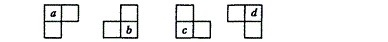
\includegraphics {2} 

Докажите, что разность между количеством уголков

вида a и количеством уголков вида b делится на 3.

\vspace { 3mm }

Ясно, что если прямоугольник m × n разрезан на уголки, то mn делится на 3. Расставим в клетках прямоугольниках числа так, как показано на рисунке.

\begin{center}

\addtolength{\tabcolsep}{-3pt}

\begin{tabular}{|c|c|c|c|c|c|c|c|c|}

\hline

1 & 2 & 3 & 4 & ... & n-3 & n-2 & n-1 & n \\

\hline

2 & 3 & 4 & 5 & ... & n-2 & n-1 & n & n+1 \\

\hline

3 & 4 & 5 & 6 & ... & n-1 & n & n+1 & n+2 \\

\hline

... & ... & ... & ... & & ... & ... & ... & ... \\

\hline

m-1&m&m+1&m+2&...&m+n-5&m+n-4&m+n-3&m+n-2\\

\hline

m & m+1 & m+2 & m+3 & ... & m+n-4 & m+n-3 & m+n-2 & m+n-1 \\

\hline

\end{tabular}

\end{center}

Сумма всех этих чисел равна $mn(m+n)/2$. Cумма чисел,

стоящих в уголке вида а, дает при делении на 3 остаток

2; сумма чисел, стоящих в уголке вида b, - остаток 1

(или, что то же самое, -2); сумма чисел, стоящих в

уголках вида с и d, делятся на 3. Если $n_a$ и $n_b$ – количества уголков вида a и вида b соответственно, то сумма

всех чисел в прямоугольнике имеет вид 3N + 2($n_a-n_b$),

где N – некоторое целое число. Из равенства.

\end{multicols}